\documentclass[11pt]{article}

\usepackage[utf8]{inputenc}
\usepackage[T1]{fontenc}
\usepackage{lmodern}
\usepackage{microtype}
\usepackage{geometry}
\geometry{margin=1in}
\usepackage{amsmath, amssymb}
\usepackage{booktabs}
\usepackage{multirow}
\usepackage{array}
\usepackage{graphicx}
\usepackage{xcolor}
\usepackage{hyperref}
\usepackage{enumitem}
\usepackage{float}
\usepackage{tikz}
\usepackage{pgfplots}
\usepgfplotslibrary{groupplots}
\usetikzlibrary{arrows.meta, positioning, shapes.geometric, fit, matrix}
\pgfplotsset{compat=1.18}

\hypersetup{
  colorlinks=true,
  linkcolor=blue,
  citecolor=blue,
  urlcolor=blue
}

\title{\textbf{Burmese-Coder-4B: Fine-Tuning a Small Language Model for Burmese Coding with Language-Aware Evaluation}}

\author{
  Wai Yan Nyein Naing \\
  \texttt{waiyan.nn18@gmail.com}
}

\date{}

\begin{document}
\maketitle

\begin{abstract}
Low-resource code generation remains underexplored, with existing benchmarks largely focused on English. Burmese coding presents a dual challenge: generating correct programs while maintaining natural Burmese explanations without corrupting programming syntax. In practice, models frequently exhibit mixed-script hallucination, unstable terminology, and cross-language token drift despite producing functionally correct code. We introduce \textbf{Burmese-Coder-4B}, a Burmese coding assistant adapted from the Gemma-3 4B family via supervised fine-tuning and Direct Preference Optimization (DPO). The alignment stage incorporates a language-aware penalization signal to suppress mixed-language outputs and improve linguistic consistency.
Evaluation is conducted using a two-track framework combining functional correctness (Pass@1) and rubric-based \textbf{LLM-as-a-Judge} scoring using Gemini 2.5 and DeepSeek V3. Burmese-Coder-4B matches the base model on Pass@1 (62.0\%) while improving rubric quality (3.779 vs.\ 3.203) and reducing mixed-language penalty (0.02 vs.\ 0.69). Compared to Qwen2.5-3B (45.0\% Pass@1, 2.526 rubric), the burmese-coder model achieves stronger alignment in both code correctness and Burmese language quality. These results demonstrate that functional correctness alone is insufficient for evaluating low-resource coding assistants. We release the model and evaluation framework to support reproducible research.\footnote{\url{https://huggingface.co/WYNN747/burmese-coder-4b}}
\end{abstract}

\section{Introduction}
Recent progress in code generation has been driven primarily by English-centric benchmarks, leaving low-resource languages substantially underexplored. Burmese presents a particularly challenging setting because coding assistants must operate across two distinct token regimes: natural-language explanation in Burmese and standardized programming syntax that should remain untranslated. In practice, this leads to a recurring failure mode in which a model may generate functionally correct code while still producing poor user-facing output through unstable terminology, mixed-script hallucination, or incorrect translation of code-related expressions.

These issues are especially pronounced in small language models and low-resource settings, where next-token generation may drift into nearby high-frequency scripts and languages observed during pretraining. As a result, conventional evaluation based only on unit-test correctness can overestimate real usability for native Burmese speakers. A model that passes tests may still fail as an assistant if its reasoning is unnatural, its terminology is inconsistent, or its explanation is contaminated by non-target scripts.

To study this gap, we present \textbf{Burmese-Coder-4B}, a Burmese coding assistant adapted from the Gemma-3 4B family through supervised fine-tuning and preference-based alignment. In parallel, we evaluate the model with a language-aware benchmark pipeline that combines functional correctness with rubric-based assessment of Burmese fluency, instruction following, terminology quality, semantic correctness, and mixed-language penalty. Results show that Burmese-Coder-4B matches the base model on Pass@1 while substantially improving Burmese-language quality, suggesting that functional correctness alone is insufficient for evaluating low-resource coding assistants.

\section{Task, Datasets, and Evaluation Framework}

\subsection{Task Setting}
We study Burmese code generation in a setting where a model must both solve programming tasks and explain code behavior in natural Burmese. This requires maintaining a clear boundary between two distinct output regimes: natural-language reasoning, which should be expressed in Burmese, and programming syntax, which should remain standard and untranslated. In practice, this distinction is non-trivial. A response may be functionally correct at the code level while still be a poor assistant for native users if its explanation is unnatural, terminologically unstable, or contaminated by non-target scripts.

\subsection{Datasets}
To support this setting, we use two complementary resources. \textbf{Burmese MBPP} serves as the supervised training corpus, teaching the model how to respond to Burmese programming instructions with code and step-by-step explanations. \textbf{Burmese HumanEval} serves as the held-out benchmark for standardized functional evaluation. These datasets play distinct roles: the former supports model adaptation, while the latter supports reproducible measurement.

This distinction is particularly important in low-resource settings. A training corpus alone cannot provide a standardized benchmark, while an evaluation set alone cannot improve model behavior in the target language. Expanding both sides therefore makes it possible to study not only whether a Burmese coding model can be trained, but also whether its improvements are measurable and comparable across future systems.

\subsection{Evaluation Framework}

A central challenge in this problem is that conventional automatic metrics do not fully capture Burmese coding quality. Unit-test metrics such as Pass@1 measure functional correctness, but they do not determine whether an explanation is natural in Burmese, faithful to the instruction, terminologically appropriate, or contaminated by non-target scripts. We considered reference-based metrics such as BLEU and chrF, but omit them from the final evaluation because they do not adequately represent either coding quality or Burmese linguistic quality in this setting.

Accordingly, we adopt a two-track evaluation framework. The first track measures \textbf{functional correctness} through unit-test execution. The second track measures \textbf{language-aware quality} through \textbf{LLM-as-a-Judge} scoring. Rather than relying on a single opaque quality label, the judge-based track evaluates responses along multiple dimensions: fluency, instruction following, semantic correctness, terminology quality, and mixed-language penalty. Together, these dimensions capture properties that directly affect native-language usability but are not observable from functional correctness alone.

% -------- FIGURE (locked position) --------
\begin{figure}[H]
\centering
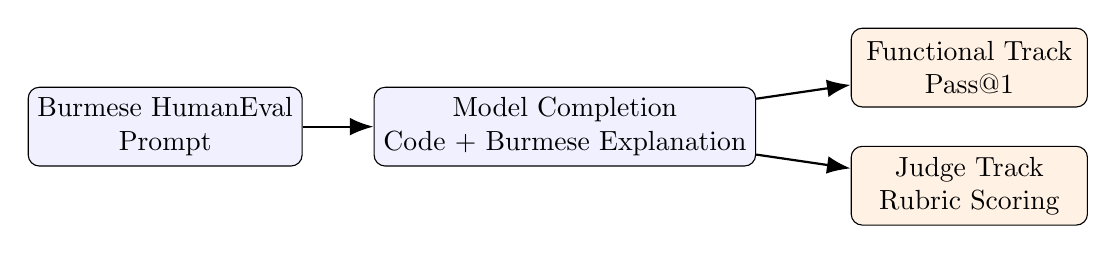
\begin{tikzpicture}[
    node distance=0.9cm and 0.9cm,
    block/.style={draw, rounded corners, align=center, minimum width=3.0cm, minimum height=1.0cm, fill=blue!6},
    metric/.style={draw, rounded corners, align=center, minimum width=3.0cm, minimum height=1.0cm, fill=orange!10},
    arrow/.style={-{Latex[length=3mm]}, thick}
]

\node[block] (prompt) {Burmese HumanEval\\Prompt};
\node[block, right=of prompt] (model) {Model Completion\\Code + Burmese Explanation};
\node[metric, right=1.2cm of model, yshift=0.75cm] (func) {Functional Track\\Pass@1};
\node[metric, right=1.2cm of model, yshift=-0.75cm] (judge) {Judge Track\\Rubric Scoring};

\draw[arrow] (prompt) -- (model);
\draw[arrow] (model) -- (func);
\draw[arrow] (model) -- (judge);

\end{tikzpicture}
\caption{Evaluation flow for Burmese coding assistants. Each model completion is assessed through two complementary tracks: functional execution and rubric-based LLM judging.}
\label{fig:eval_flow}
\end{figure}

To make the judge-based track interpretable, we score each response along multiple dimensions rather than using a single undifferentiated quality score. These dimensions reflect properties that matter for native Burmese users in practical coding assistance: whether the explanation reads naturally, follows the instruction, preserves the intended program logic, uses appropriate technical terminology, and avoids contamination from non-target scripts. The aggregate rubric score is computed as

\begin{equation}
\text{Rubric Score} =
\frac{
\text{Fluency} +
\text{Instruction Following} +
\text{Semantic Correctness} +
\text{Terminology}
}{4}
- \text{Mix Penalty}.
\label{eq:rubric_score}
\end{equation}

This formulation treats mixed-language contamination as an explicit penalty rather than folding it into a generic quality average. As a result, the reported rubric score reflects both positive language quality and robustness against a key low-resource failure mode.

\begin{table}[H]
\centering
\small
\renewcommand{\arraystretch}{1.2}
\caption{Dimensions used in the judge-based evaluation framework. Higher is better except Mix Penalty.}
\label{tab:rubric_dimensions}
\begin{tabular}{|p{5cm}|p{8cm}|}
\hline
\textbf{Dimension} & \textbf{Description} \\
\hline
Fluency & Measures whether the Burmese explanation is natural, readable, and well-formed for a native speaker. \\
\hline
Instruction Following & Evaluates whether the response faithfully follows the Burmese instruction, including both code behavior and explanation. \\
\hline
Semantic Correctness & Assesses whether the explanation and generated solution are logically aligned with the intended task. \\
\hline
Terminology & Checks whether programming concepts are expressed using appropriate and consistent Burmese technical terms. \\
\hline
Mix Penalty & Measures contamination by foreign-language or foreign-script tokens (lower is better). \\
\hline
\end{tabular}
\end{table}

Publicly discussed Burmese coding baselines and standardized evaluation pipelines remain scarce. This makes it difficult to compare localized Burmese coding models under a shared protocol and difficult to separate real improvements from anecdotal examples. The framework used in this work addresses this gap by pairing a Burmese adaptation of HumanEval with a reusable evaluation suite that supports unit-test evaluation and OpenAI-compatible LLM-as-a-Judge scoring through a unified workflow.

\section{Model Adaptation}
We adapt the Gemma-3 4B family in two stages. The first stage uses \textbf{supervised fine-tuning (SFT)} on Burmese programming instruction data to teach the model how to generate code and explain it in Burmese. The second stage applies \textbf{Direct Preference Optimization (DPO)} to reduce multilingual drift and improve linguistic stability.

\begin{figure}[H]
\centering
\resizebox{\linewidth}{!}{%
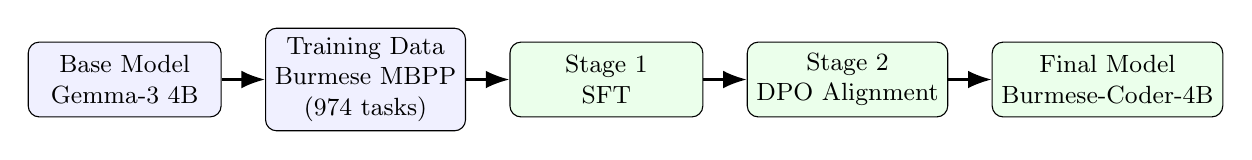
\begin{tikzpicture}[
    font=\small,
    node distance=0.55cm and 0.55cm,
    block/.style={draw, rounded corners, align=center, minimum width=2.45cm, minimum height=0.95cm, fill=green!8},
    data/.style={draw, rounded corners, align=center, minimum width=2.45cm, minimum height=0.95cm, fill=blue!6},
    arrow/.style={-{Latex[length=3mm]}, thick}
]

\node[data] (base) {Base Model\\Gemma-3 4B};
\node[data, right=of base] (mbpp) {Training Data\\Burmese MBPP\\(974 tasks)};
\node[block, right=of mbpp] (sft) {Stage 1\\SFT};
\node[block, right=of sft] (dpo) {Stage 2\\DPO Alignment};
\node[block, right=of dpo] (final) {Final Model\\Burmese-Coder-4B};

\draw[arrow] (base) -- (mbpp);
\draw[arrow] (mbpp) -- (sft);
\draw[arrow] (sft) -- (dpo);
\draw[arrow] (dpo) -- (final);

\end{tikzpicture}%
}
\caption{Two-stage adaptation pipeline for Burmese-Coder-4B. The base Gemma-3 4B model is first adapted with supervised fine-tuning on Burmese MBPP, then aligned with DPO to reduce mixed-language drift and improve Burmese response quality.}
\label{fig:train_flow}
\end{figure}

The SFT stage uses a Burmese MBPP-style dataset containing \textbf{974 programming tasks}. Each instance includes a Burmese instruction, a Python solution, and a Burmese explanation of the code logic. This stage primarily teaches the model how to structure technical responses in Burmese rather than only emit code.

The SFT implementation uses parameter-efficient fine-tuning with \textbf{LoRA}, where low-rank adapter weights are trained instead of updating the full base model. The core setup uses context length 2048, 4-bit loading, LoRA rank 16, LoRA alpha 16, batch size 16, gradient accumulation 4, learning rate \(2 \times 10^{-4}\), and 15 warmup steps.

After SFT, we apply DPO to improve linguistic stability. DPO is a preference-based alignment method in which the model learns to prefer a better response over a worse response for the same prompt. In this work, the preferred response is the cleaner Burmese response, while the rejected response contains undesirable behaviors such as script mixing, hallucinated foreign tokens, or less stable technical phrasing. The DPO stage uses context length 2048, 4-bit loading, batch size 2, gradient accumulation 16, learning rate \(3 \times 10^{-6}\), 300 max steps, and \(\beta = 0.5\). Here, \(\beta\) controls how strongly the model is pushed to prefer the chosen response over the rejected one; we use a relatively strong value to make mixed-language penalties more effective.

\section{Experimental Setup}
We evaluate on \textbf{Burmese HumanEval}, a Burmese adaptation of HumanEval containing \textbf{100 programming problems}. Each task provides a Burmese prompt and hidden unit tests. We compare three systems: \textbf{burmese-coder-4b} (ours), \textbf{gemma3\_4b} (base model), and \textbf{qwen2.5\_3b}.

The evaluation framework uses two complementary tracks:
\begin{itemize}[leftmargin=1.2cm]
    \item \textbf{Functional track:} unit-test execution with Pass@1.
    \item \textbf{Judge track:} rubric-based scoring with an LLM judge.
\end{itemize}

The judge track measures qualities that are difficult to capture with conventional metrics alone, including Burmese fluency, instruction following, semantic correctness, terminology quality, and mixed-language penalty. Rubric scores are reported using two separate LLM judges: DeepSeek V3 and Gemini 2.5. The judge interface is OpenAI-compatible, making the framework portable across different model backends.

The end-to-end training was run on an H100 GPU on RunPod cloud infrastructure and cost approximately USD 40 over about 2.75 hours.

\section{Results}
Table~\ref{tab:main_results} and Figure~\ref{fig:benchmark_chart} present the main benchmark comparison. The key result is that Burmese-Coder-4B matches the base Gemma model on functional correctness while achieving substantially better Burmese-language quality under rubric-based evaluation. This pattern is consistent across both LLM judges and is especially visible in the mixed-language penalty, where the aligned model exhibits far less cross-script contamination.

\begin{figure}[t]
\centering
\begin{tikzpicture}
\begin{groupplot}[
    group style={
        group size=2 by 2,
        horizontal sep=1.4cm,
        vertical sep=2.0cm
    },
    width=0.44\linewidth,
    height=0.30\linewidth,
    ybar,
    bar width=9pt,
    ymin=0,
    enlarge x limits=0.30,
    symbolic x coords={bc4b,gemma,qwen},
    xtick=data,
    xticklabels={Burmese\\Coder,Gemma-3\\4B,Qwen2.5\\3B},
    x tick label style={
        align=center,
        font=\small,
        text depth=0.15em
    },
    tick label style={font=\small},
    label style={font=\small},
    title style={font=\small},
    ymajorgrids=true,
    grid style={dashed, gray!25},
    axis line style={black!60},
    tick style={black!60},
]

\nextgroupplot[
    title={Pass@1},
    ylabel={Score},
    ymin=0, ymax=100
]
\addplot[fill=blue!70, draw=black] coordinates {
    (bc4b,62)
    (gemma,62)
    (qwen,45)
};

\nextgroupplot[
    title={Rubric Score},
    ymin=0, ymax=4
]
\addplot[fill=blue!70, draw=black] coordinates {
    (bc4b,3.456)
    (gemma,2.939)
    (qwen,1.220)
};
\addplot[fill=orange!80, draw=black] coordinates {
    (bc4b,3.779)
    (gemma,3.203)
    (qwen,2.526)
};

\nextgroupplot[
    yshift=-10pt,
    title={Mix Penalty ($\downarrow$ better)},
    ylabel={Penalty},
    ymin=0, ymax=1.5
]
\addplot[fill=blue!70, draw=black] coordinates {
    (bc4b,0.09)
    (gemma,0.72)
    (qwen,1.18)
};
\addplot[fill=orange!80, draw=black] coordinates {
    (bc4b,0.02)
    (gemma,0.69)
    (qwen,1.37)
};

\nextgroupplot[
    hide axis
]

\end{groupplot}

\node at ($(group c1r1.north)!0.5!(group c2r1.north)+(0,1.1cm)$) {
\begin{tikzpicture}
\matrix[
    matrix of nodes,
    row sep=0.2cm,
    column sep=0.5cm,
    nodes={anchor=west, font=\small}
]{
    \draw[fill=blue!70, draw=black] (0,0) rectangle (0.28,0.16); & DeepSeek &
    \draw[fill=orange!80, draw=black] (0,0) rectangle (0.28,0.16); & Gemini \\
};
\end{tikzpicture}
};

\end{tikzpicture}
\caption{Benchmark results on Burmese coding evaluation. Top-left: functional correctness measured by Pass@1. Top-right: overall rubric score from two LLM judges. Bottom-left: mixed-language penalty, where lower is better. Burmese-Coder-4B matches the base Gemma-3 4B model on Pass@1 while achieving higher rubric scores and substantially lower cross-language mixing.}
\label{fig:benchmark_chart}
\end{figure}

\begin{table}[t]
\centering
\small
\caption{Main benchmark comparison on Burmese coding evaluation. Higher is better except Mix Penalty.}
\label{tab:main_results}
\begin{tabular}{lccc}
\toprule
Model & Pass@1 (\%) & Rubric (DeepSeek) & Rubric (Gemini) \\
\midrule
burmese-coder-4b & \textbf{62.0} & \textbf{3.456} & \textbf{3.779} \\
gemma3\_4b       & 62.0          & 2.939          & 3.203 \\
qwen2.5\_3b      & 45.0          & 1.220          & 2.526 \\
\bottomrule
\end{tabular}
\end{table}

\begin{table}[t]
\centering
\small
\caption{Detailed rubric breakdown under DeepSeek judge. Higher is better except Mix Penalty.}
\label{tab:deepseek_breakdown}
\begin{tabular}{lccccc}
\toprule
Model & Fluency & Instr. & Semantic & Terminology & Mix Penalty \\
\midrule
burmese-coder-4b & \textbf{3.82} & \textbf{3.43} & \textbf{3.26} & \textbf{3.62} & \textbf{0.09} \\
gemma3\_4b       & 3.52          & 3.26          & 2.95          & 3.18          & 0.72 \\
qwen2.5\_3b      & 1.75          & 1.28          & 1.16          & 1.45          & 1.18 \\
\bottomrule
\end{tabular}
\end{table}

\begin{table}[t]
\centering
\small
\caption{Detailed rubric breakdown under Gemini judge. Higher is better except Mix Penalty.}
\label{tab:gemini_breakdown}
\begin{tabular}{lccccc}
\toprule
Model & Fluency & Instr. & Semantic & Terminology & Mix Penalty \\
\midrule
burmese-coder-4b & \textbf{3.98} & \textbf{3.78} & \textbf{3.55} & \textbf{3.92} & \textbf{0.02} \\
gemma3\_4b       & 3.71          & 3.66          & 3.16          & 3.49          & 0.69 \\
qwen2.5\_3b      & 2.40          & 2.41          & 3.08          & 3.19          & 1.37 \\
\bottomrule
\end{tabular}
\end{table}

Across both LLM judges, the most striking improvement is the reduction in mixed-language contamination. Under Gemini, the mix penalty decreases from 0.69 for the base Gemma model to 0.02 for Burmese-Coder-4B. Under DeepSeek, it decreases from 0.72 to 0.09. At the same time, the fine-tuned model improves fluency, terminology, and semantic alignment while preserving the same Pass@1 as the base model.

\section{Analysis}
The results suggest that the primary benefit of adaptation is not a large increase in raw code-solving ability, but a substantial improvement in linguistic reliability. Supervised fine-tuning improves the model's ability to structure Burmese explanations and follow Burmese instructions, while preference-based alignment appears to be the main driver of reduced mixed-script hallucination. This explains why the fine-tuned model can remain comparable on Pass@1 yet feel significantly better for native users.

More broadly, these findings indicate that functional correctness alone can mask important usability differences in low-resource coding assistants. In Burmese, a model can solve the task while still failing at the explanation layer through unstable terminology, unnatural phrasing, or multilingual drift. Language-aware evaluation is therefore not an auxiliary feature, but a necessary part of the measurement protocol.

A representative qualitative example further supports this pattern. When asked to organize files into folders, the untuned Gemma response mixed Burmese with fragments from other writing systems in both the explanatory text and surrounding instruction. By contrast, Burmese-Coder-4B produced a cleaner and more consistent response while keeping the code in standard Python. This qualitative difference aligns with the large drop in mix penalty observed in the benchmark tables.

\section{Limitations}
This study has several limitations. First, the training dataset is still relatively small for code modeling. Second, evaluation is centered on Python and HumanEval-style tasks rather than broader software engineering workflows such as repositories, debugging, tool use, or long-horizon coding assistance. Third, rubric-based evaluation depends on judge models, which may themselves introduce bias or variance. Finally, while the results indicate reduced multilingual drift, the exact token-level causes of this phenomenon remain an open research question.

\section{Conclusion}
We introduced Burmese-Coder-4B, a compact Burmese coding assistant trained with supervised fine-tuning and preference-based alignment. Although the model does not outperform the base Gemma model on Pass@1, it produces substantially better Burmese-language explanations, better terminology usage, and far lower mixed-language contamination. These findings show that localized coding assistants should be evaluated not only by code correctness, but also by how well they communicate with users in the target language.

\begin{thebibliography}{9}

\bibitem{chen2021codex}
Mark Chen et al.
\newblock Evaluating Large Language Models Trained on Code.
\newblock \emph{arXiv preprint arXiv:2107.03374}, 2021.

\bibitem{burmese_humaneval}
Wai Yan Nyein Naing.
\newblock Burmese HumanEval: A Benchmark for Evaluating Burmese Coding Assistants.
\newblock Hugging Face dataset, 2026.
\newblock \url{https://huggingface.co/datasets/WYNN747/burmese-human-eval}

\bibitem{burmese_mbpp}
Wai Yan Nyein Naing.
\newblock Burmese MBPP: A Large-Scale Programming Dataset for Burmese Coding Assistants.
\newblock Hugging Face dataset, 2026.

\bibitem{burmese_coding_eval}
Wai Yan Nyein Naing.
\newblock Burmese-Coding-Eval: A Translated and Expanded HumanEval Benchmark for Burmese Programming Assistants.
\newblock GitHub repository, 2026.
\newblock \url{https://github.com/WaiYanNyeinNaing/burmese-coding-eval}

\bibitem{dpo}
Rafael Rafailov et al.
\newblock Direct Preference Optimization: Your Language Model is Secretly a Reward Model.
\newblock \emph{arXiv preprint arXiv:2305.18290}, 2023.

\end{thebibliography}

\end{document}